\documentclass[12pt]{book}

\usepackage[dvips,letterpaper,margin=0.75in,bottom=0.5in]{geometry}
\usepackage{cite}
\usepackage{slashed}
\usepackage{graphicx}
\usepackage{amsmath}
\usepackage{amssymb}
\usepackage{braket}
\begin{document}

\newcommand{\ihbar}{\ensuremath{i \hbar}}
\newcommand{\Pss}{\ensuremath{\Psi^*}}
\newcommand{\dPsidt}{\ensuremath{ \frac{\partial \Psi}{\partial t} }}
\newcommand{\dPsidx}{\ensuremath{ \frac{\partial \Psi}{\partial x} }}
\newcommand{\ddPsidx}{\ensuremath{ \frac{\partial^2 \Psi}{\partial x^2} }}
\newcommand{\dPssdt}{\ensuremath{ \frac{\partial \Psi^*}{\partial t} }}
\newcommand{\dPssdx}{\ensuremath{ \frac{\partial \Psi^*}{\partial x} }}
\newcommand{\ddPssdx}{\ensuremath{ \frac{\partial^2 \Psi^*}{\partial x^2} }}

\newcommand{\dphidt}{\ensuremath{ \frac{d \phi}{dt} }}
\newcommand{\dpsidx}{\ensuremath{ \frac{d \psi}{dx} }}
\newcommand{\ddpsidx}{\ensuremath{ \frac{d^2 \psi}{dx^2} }}


\title{PHY 115A \\ Lecture Notes: \\ 
Fourier Series and Fourier Transform \\}
\author{Michael Mulhearn}

\maketitle

\appendix
\setcounter{chapter}{5}
\chapter{Fourier Series and Fourier Transform}

\section{The Fourier Series}

In this section, we'll see how the Fourier Series can be interpreted in the context of a vector space with an inner product.  

\subsection{Vector Spaces and Inner Product Spaces}
The real numbers ($\mathbb{R}$) and complex numbers ($\mathbb{C}$) are both examples of fields in mathematics:  they are each a set on which the operations addition, subtraction, multiplication, and division are defined and follow their familiar rules.  A vector space $V$ over a scalar field $S$ is a set whose elements are called vectors, for which an associative and commutative operation of addition and an associative and distributive operation of scalar multiplication are both defined.    The complete set of properties which define a vector field are shown in Table~\ref{tbl:ipspace}.  

An {\em inner product} is an operation which returns a scalar for any two vectors $x$ and $y$.
We write the inner product as $\braket{x|y}$.  If a vector space $V$ has an inner product defined 
which satisfies conditions I1-I5 in the table, it is an inner product space $H$ as well.  It is left as an exercise to show that the deducible properties D1-D4 listed in the table follow from the other properties.

\begin{table}
\caption{ \label{tbl:ipspace} Here we define the properties of a vector space $V$ over a scalar field $S$, and an inner product space $H$ as well, using a compact mathematical notation.  In this class the scalar field $S$ will only be the real numbers ($\mathbb{R}$) or the complex numbers ($\mathbb{C}$).
When $S=\mathbb{R}$, just ignore all complex conjugation below, e.g. take $\alpha^* = \alpha$.}
\begin{center}
{\bf Useful Math Symbols:}\\
\begin{tabular}{ll}
  $\forall \, x \in V$ & for all $x$ in $V$ (for any vector $x$)\\
  $\forall \, \alpha \in S$ & for all $\alpha$ in $S$ (for any scalar $\alpha$) \\
%  $\exists y$ & there exists $y$ \\
  $\exists ! \, y$ & there exists unique $y$ \\
  s.t.          & such that \\
\end{tabular}\\    
\vskip 0.5cm
{\bf Properties of Addition:}\\
\begin{tabular}{llll}
{\bf A1} & {\bf Closure} & $\forall x,y \in V$ & $(x+y) \in V $\\
{\bf A2} & {\bf Commutative} & $\forall x,y \in V$ & $x+y=y+z$\\
{\bf A3} & {\bf Associative} & $\forall x,y,z \in V$ & $(x+y)+z = x+(y+z)$\\
{\bf A4} & {\bf Zero}        & $\exists !~0$~~s.t.~~ $\forall x \in V$ & $x+0 = x$ \\
{\bf A5} & {\bf Inverse} & $\forall x \in V \exists !\;(-x) \in V$~~s.t.~~& $x+(-x)=0$\\
\end{tabular} \\
\vskip 0.5cm
{\bf Properties of Scalar Multiplication:}\\
\begin{tabular}{llll}
  {\bf M1} & {\bf Closure} & $\forall x \in V$ and $\forall \alpha \in S$ & $\alpha x \in V$\\
  {\bf M2} & {\bf Identity} & $\forall x \in V$ & $1x=x$\\
  {\bf M3} & {\bf Associative} & $\forall x \in V$
and $\forall \alpha,\beta \in S$ & $\alpha(\beta x) = (\alpha \beta) x$\\
{\bf M4} & {\bf Distributive} & $\forall x,y \in V$and $\forall \alpha \in S$ & $\alpha(x+y) = \alpha x + \alpha y$ \\
  {\bf M5} & {\bf Distributive} & $\forall x \in V$and $\forall \alpha,\beta \in S$ & $ (\alpha + \beta)x = \alpha x + \beta x $ \\
\end{tabular}
\vskip 0.5cm
{\bf Deducible Properties:}\\
\begin{tabular}{lll}
{\bf D1}  & $\forall x \in V $  & $0x = 0$ \\
{\bf D2}  & $\forall x \in V $  & $(-1)x = (-x)$ \\
\end{tabular}
\vskip 0.5cm
{\bf Properties of Inner Products:}\\
\begin{tabular}{lll}
  {\bf I1} & $\forall x,y \in H$ & $\braket{x|y}^* = \braket{y|x}$\\
{\bf I2} & $\forall x,y,z \in H$and $\forall \alpha \in S$ &
$\braket{x|\alpha y} = \alpha \braket{x|y}$\\
{\bf I3} & $\forall x,y,z \in H$ & $\braket{x+y|z} = \braket{x|z}+\braket{y|z}$\\
{\bf I4} & $\forall x \in H$ & $\braket{x|x} \geq 0$ \\
{\bf I5} & $\forall x \in H$ & $\braket{x|x}=0$ if and only if $x=0$ \\
\end{tabular}
\vskip 0.5cm
{\bf Deducible Properties:}\\
\begin{tabular}{llll}
{\bf D3} & & $\forall x,y \in H$and $\forall \alpha \in S$ &
$\braket{\alpha x|y} = \alpha^* \braket{x|y}$\\
{\bf D4} & & $\forall x,y,z \in H$ &
$\braket{x|y+z} = \braket{x|y}+\braket{x|z}$\\
\end{tabular}
\end{center}
\end{table}

\subsection{Euclidean Vector Space}

Before turning to the Fourier Series, let's explore how the properties of an abstract vector space apply to the familiar Euclidean vectors.  Such a vector is completely specified by its displacement in each spatial direction.  Let's see how the axiomatic properties of Table~\ref{tbl:ipspace} apply in this case. Note that the scalar field $S$ is the real numbers ($\mathbb{R}$), so we'll just ignore all complex conjugation in the table for now.

\begin{samepage}
We have {\bf vector addition} which satisfies properties A1-A5 of Table~\ref{tbl:ipspace}:
\begin{itemize}
\item {\bf A1}: $\vec{u} + \vec{v} = \vec{w}$ 
\item {\bf A2}: $\vec{v} + \vec{w} = \vec{w} + \vec{v}$
\item {\bf A3}: $\vec{u} + (\vec{v} + \vec{w}) = (\vec{u} + \vec{v}) + \vec{w} $
\item {\bf A4}: There is the vector 0 with: $\vec{v} + 0 = \vec{v} $
\item {\bf A5}: For every $\vec{v}$ there is $(-\vec{v})$ s.t $\vec{v} + (-\vec{v}) = 0$
\end{itemize}
\end{samepage}

\begin{samepage}
\noindent
We also have {\bf scalar multiplication} which satisfies properties M1-M5 and D1,D2:
\begin{itemize}
\item {\bf M1:} $a \vec{v} = \vec{w}$
\item {\bf M2:} $1 \vec{v} = \vec{v}$
\item {\bf M3:} $a(b\vec{v}) = (ab)\vec{v}$
\item {\bf M4:} $a(\vec{v} + \vec{w}) = a\vec{v} + a\vec{w}$
\item {\bf M5:} $(a+b)\vec{v} = a\vec{v} + b\vec{v}$
\item {\bf D1:} $(-1)\vec{v} = (-\vec{v})$
\item {\bf D2:} $0\vec{v} = 0$
\end{itemize}
\end{samepage}

\noindent
In this vector space, the dot product:
\begin{displaymath}
\vec{v} \cdot \vec{w} = v_x w_x + v_y w_y + v_z w_z 
\end{displaymath}
is the inner product which satisfies properties I1-I5:
\begin{itemize}
\item {\bf I1:} $\vec{v} \cdot \vec{w} = \vec{w} \cdot \vec{v}$
\item {\bf I2:} $\vec{v} \cdot \left(a\vec{w}\right) = a \vec{v} \cdot \vec{w}$
\item {\bf I3:} $\left(\vec{u} + \vec{v}\right) \cdot \vec{w} = \vec{u} \cdot \vec{w} + \vec{v} \cdot \vec{w} $
\item {\bf I4:} $\vec{v} \cdot \vec{v} \geq 0$
\item {\bf I5:} $\vec{v} \cdot \vec{v} = 0$ if and only if $\vec{v} = 0$
\item {\bf D3:} $\left(a\vec{v}\right) \cdot \vec{w} = a \left( \vec{v} \cdot \vec{w}\right) $
\item {\bf D4:} $\vec{w} \cdot \left(\vec{u} + \vec{v}\right)  = \vec{w} \cdot \vec{u} + \vec{w} \cdot \vec{v}$
\end{itemize}

\noindent
We have a set of {\em basis vectors}: $\hat{x}$, $\hat{y}$, and $\hat{z}$.  These basis vectors are orthogonal:
\begin{displaymath}
\hat{x} \cdot \hat{y} = \hat{y} \cdot \hat{z} = \hat{z} \cdot \hat{x} = 0
\end{displaymath}
and normalized:
\begin{displaymath}
\hat{x} \cdot \hat{x} = \hat{y} \cdot \hat{y} = \hat{z} \cdot \hat{z} = 1.
\end{displaymath}
When the basis vectors have both of these properties, we call them {\em orthonormal}.

For any possible vector $\vec{v}$, we can calculate its component in the direction of each basis vector by calculating the inner product:
\begin{eqnarray*}
v_x = \vec{v} \cdot \hat{x} \\
v_y = \vec{v} \cdot \hat{y} \\
v_z = \vec{v} \cdot \hat{z} \\
\end{eqnarray*}
We say that the basis vectors $\hat{x}$, $\hat{y}$, and $\hat{z}$ are ``complete'', because specifying the values of $v_x$, $v_y$, and $v_z$ completely describes the vector $v$.  (Alternatively, we can say that the basis vectors span the vector space $V$.)  The set of basis vectors $\hat{x}$ and $\hat{z}$ are orthonormal, but they are not complete in three dimensional space, because there are vectors which we cannot write using only these two directions.  For instance, there are no possible values for $v_x$ and $v_z$
which make
\begin{eqnarray*}
 \vec{v_1} = v_x \hat{x} + v_z \hat{z}
\end{eqnarray*}
equal to the vector
\begin{eqnarray*}
 \vec{v_2} = 3 \hat{x} + 2 \hat{y} + 7 \hat{z}.
\end{eqnarray*}
Orthogonality and completeness are intimately related.  In Euclidean vector space, any three orthogonal vectors are a complete basis.
 
\subsection{The Fourier Series}

Using the language of inner product spaces, the Fourier Theorem states that the sines and cosines form a complete orthonormal basis for any periodic function.  The vectors in this vector space are periodic functions.  Addition of periodic functions $f(x)$ and $g(x)$ is another periodic function $f(x) + g(x)$.  Scalar multiplication of a periodic function $f(x)$ by a real number $a$ is another periodic function $a f(x)$.  The other properties of vector addition and scalar multiplication follow from the corresponding rules of ordinary addition and multiplication.

To obtain an inner product space, we need to define the inner product. If we restrict ourselves to {\bf real} functions of $x$ with period $a$, the inner product between any two functions $f(x)$ and $g(x)$ is defined to be the integral:
\begin{equation}
\braket{f|g} \equiv \int_{-\frac{a}{2}}^{\frac{a}{2}} f(x) \, g(x) \, dx
\end{equation}
The basis vectors are the sine and cosine functions
\begin{eqnarray}
s_n(x) &\equiv& \sqrt{\frac{2}{a}}\,\sin\left(\frac{2\pi n}{a} \, x \right)\\
c_n(x) &\equiv& \sqrt{\frac{2}{a}}\,\cos\left(\frac{2\pi n}{a} \, x \right)
\end{eqnarray}
which are defined for
\begin{eqnarray*}
n = 1,2,3,...
\end{eqnarray*}
plus the constant function:
\begin{eqnarray}
c_0(x) \equiv \sqrt{\frac{1}{a}}
\end{eqnarray}
Note that if it existed, $s_0(x) = 0$ would not be normalizable.

We leave it as an exercise to show that:
\begin{eqnarray}
\braket{s_n | s_m} &=& \delta_{nm}\notag\\[8pt]
\braket{c_n | c_m} &=& \delta_{nm}\notag\\[8pt]
\braket{s_n | c_m} &=& 0\notag\\[8pt]
\end{eqnarray}
for all $n$ and $m$, but take care that $c_0$ exists while $s_0$ does not.  
For compact notation we use the Kronecker delta symbol:
\begin{displaymath}
\delta_{nm} =  
\left\{
	\begin{array}{ll}
		1  & \mbox{if } n=m \\
		0 & \mbox{otherwise}
	\end{array}
\right.
\end{displaymath}
We can write the orthonormality conditions out explicitly as integrals for $n>0$ and $m>0$ as:
\begin{eqnarray}
\braket{s_n|s_m} &=& \frac{2}{a} \int_{-\frac{a}{2}}^{\frac{a}{2}} 
\sin\left(\frac{2\pi n}{a} \, x \right) \sin\left(\frac{2\pi m}{a} \, x \right) \, dx = \delta_{nm} \;\;\;\;\; \notag\\[8pt]
\braket{c_n| c_m} &=& \frac{2}{a} \int_{-\frac{a}{2}}^{\frac{a}{2}} 
\cos\left(\frac{2\pi n}{a} \, x \right) \cos\left(\frac{2\pi m}{a} \, x \right) \, dx = \delta_{nm}\notag\\[8pt]
\braket{s_n| c_m} &=& \frac{2}{a} \int_{-\frac{a}{2}}^{\frac{a}{2}} 
\sin\left(\frac{2\pi n}{a} \, x \right) \cos\left(\frac{2\pi m}{a} \, x \right) \, dx = 0 \notag\\
\end{eqnarray}
leaving the special case for $c_0$ (and still keeping $n>0$):
\begin{eqnarray}
\braket{c_n| c_0} &=& \frac{\sqrt{2}}{a} \int_{-\frac{a}{2}}^{\frac{a}{2}} 
\cos\left(\frac{2\pi n}{a} \, x \right) \, dx = 0 \notag\\[8pt]
\braket{s_n| c_0} &=& \frac{\sqrt{2}}{a} \int_{-\frac{a}{2}}^{\frac{a}{2}} 
\sin\left(\frac{2\pi n}{a} \, x \right) \, dx = 0 \notag\\
\braket{c_0| c_0} &=& \frac{1}{a} \int_{-\frac{a}{2}}^{\frac{a}{2}} dx = 1 \notag\\
\end{eqnarray}
Fourier's Theorem states that these orthonormal basis functions are complete for the vector space of periodic functions with period $a$.  That is, if $f(x)$ has the property that:
$$f(x) = f(x+a)$$
then $f(x)$ can be written as a sum of the orthonormal basis vectors:
\begin{equation}
f(x) \; = \; \sum_{n=0}^{\infty}  A_n \, c_n(x)  \; \; + \; \; \sum_{n=1}^{\infty} B_n \, s_n(x) \label{eqn:bfs}
\end{equation}
or explicitly in terms of sine and cosine functions:
\begin{equation}
f(x) = A_0 \sqrt{\frac{1}{a}} + \sqrt{\frac{2}{a}} \sum_{n=1}^{\infty}  \left[ A_n \, \cos\left(\frac{2\pi n}{a} \, x \right) + B_n \, \sin\left(\frac{2\pi n}{a} \, x \right)\right]\label{eqn :lfs}
\end{equation}
The values $A_n$ and $B_n$ are called {\em Fourier coefficients}.  The $N$th term in the Fourier Series refers to the approximation for $f(x)$ from the first $N$ terms in the infinite sum above, and we say that the Fourier Series converges to the function $f(x)$.  The demonstration of completeness is optional reading, available in the Appendix.

\begin{figure}[thb]
\begin{center}
{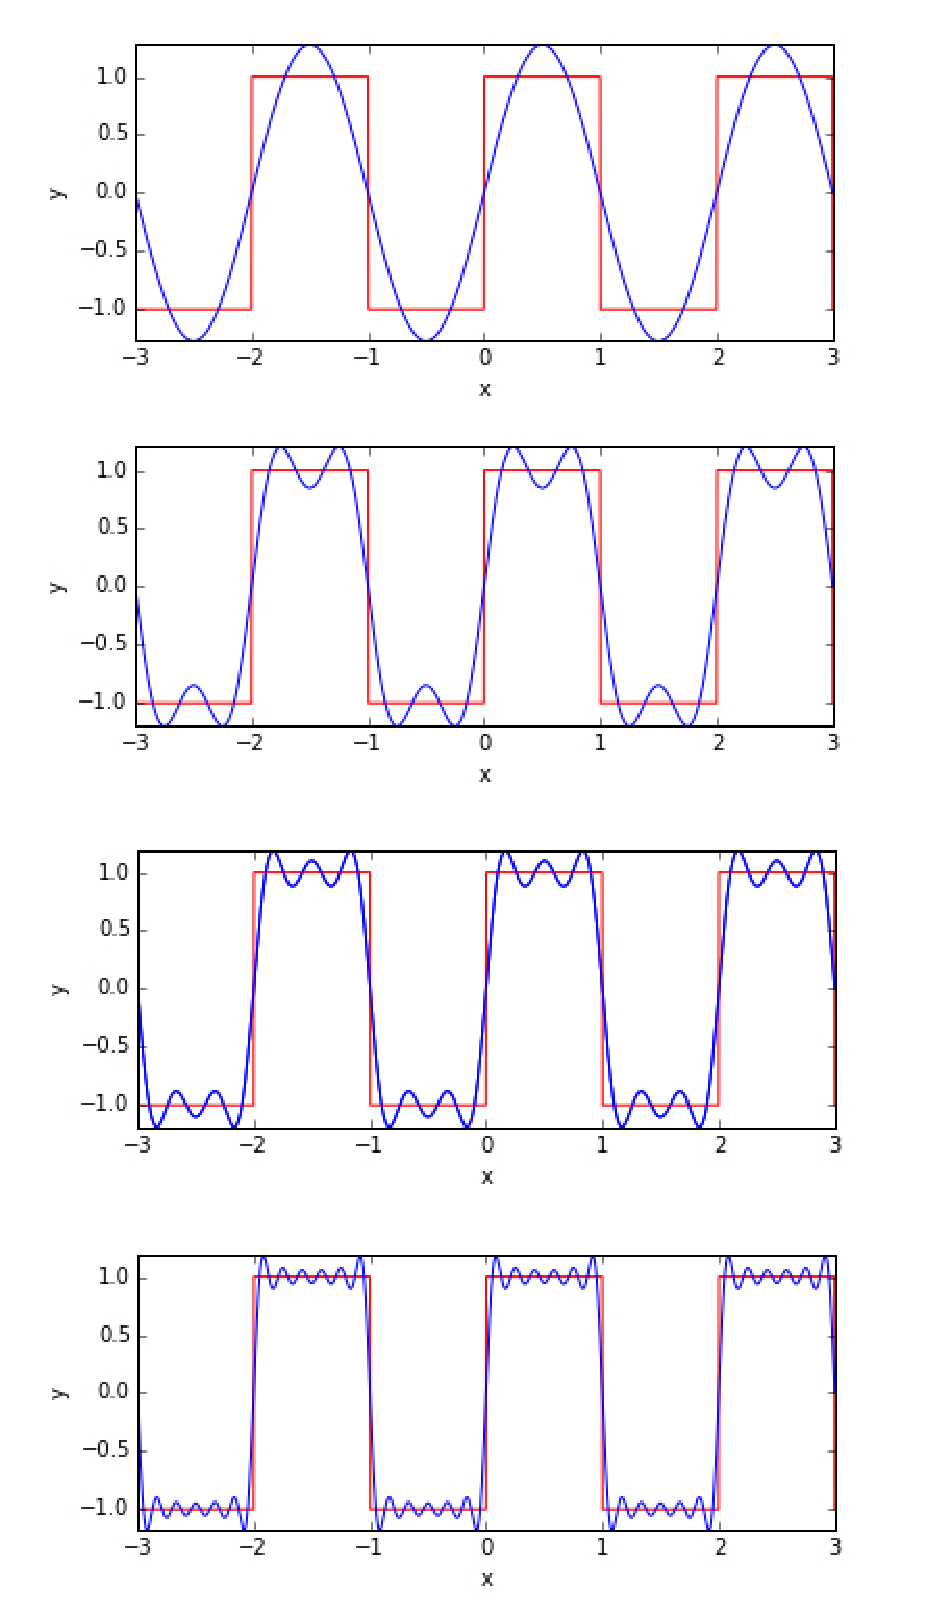
\includegraphics[width=0.40\textwidth]{figs/fsall.pdf}}
\end{center}
\caption{\label{fig:fall} The Fourier Series for a step function including one term, three terms, five terms, and nineteen terms.  The Fourier Theorem states that the series will converge, reproducing the original function, as the number of terms approaches infinity.}
\end{figure}

For a visual example of the Fourier Series, the first terms of the Fourier Series for a step function are shown in Fig.~\ref{fig:fall}.  

\subsection{Determining Fourier Coefficients}
\label{sect:coeff}

Just as in the Euclidean vector space, we can determine the Fourier coefficients of a function $f$ by computing the inner products:
\begin{eqnarray*}
A_n = \braket{c_n| f} \\
B_n = \braket{s_n| f}
\end{eqnarray*}
or, in terms of the inner product integrals and sine and cosine functions:
\begin{eqnarray*}
A_0 &=& \sqrt{\frac{1}{a}} \int_{-\frac{a}{2}}^{\frac{a}{2}} f(x) \, dx \\
A_n &=& \sqrt{\frac{2}{a}} \int_{-\frac{a}{2}}^{\frac{a}{2}} 
\cos\left(\frac{2\pi n}{a} \, x \right) \, f(x) \, dx \\
B_n &=& \sqrt{\frac{2}{a}} \int_{-\frac{a}{2}}^{\frac{a}{2}} 
\sin\left(\frac{2\pi n}{a} \, x \right) \, f(x) \, dx \\
\end{eqnarray*}


The inner product determines the correct coefficients only because the basis functions are complete and orthonormal.  To see how this works, start with the completeness equation but replace $n$ with $m$ for clarity later:
\begin{equation*}
f(x) \; = \; \sum_{m=0}^{\infty}  A_m \, c_m(x)  \; \; + \; \; \sum_{m=1}^{\infty} B_m \, s_m(x)
\end{equation*}
Then calculate:
\begin{eqnarray*}
  \braket{c_n| f} \; &=& \; \braket{c_n | \sum_{m=0}^{\infty}  A_m \, c_m  \; \; + \; \; \sum_{m=1}^{\infty} B_m \, s_m }\\[8pt]
  &=& \; \sum_{m=0}^{\infty}  A_m \, \braket{c_n| c_m}  \; \; + \; \; \sum_{m=1}^{\infty} B_m \, \braket{c_m| s_m} \\[8pt]
 &=& \; \sum_{m=0}^{\infty}  A_m \; \delta_{nm}  \; \; + \; \; \sum_{m=1}^{\infty} B_m \; 0 \\[8pt]
\braket{c_n| f} \; &=& A_n \\
\end{eqnarray*}
Note that the second step follows from properties I2 and D4 of
Table~\ref{tbl:ipspace}.  In the last step the only non-zero value in
the sum across $m$ is the term for $m=n$, because of the
$\delta_{nm}$.  It is left as an exercise to work this out for
$\braket{s_n | f}$.  (It is also helpful to work through these same
steps using the integral form of the orthogonality conditions.  It's
much more cumbersome notation, but much more explicit about what is
going on.  I highly recommend doing this if you are finding the
abstract notation confusing at this point.)

\subsection{Fourier Series for Complex Functions}

The Fourier series for a periodic function with period $a$ can be expressed in terms of the complex exponential by noting that:
\begin{eqnarray*}
\sin\theta \; = \; \frac{e^{i \theta} - e^{-i \theta}}{2i} \\[5pt]
\cos\theta \; = \; \frac{e^{i \theta} + e^{-i \theta}}{2} \\
\end{eqnarray*}
Later in the Appendix, we determine the Fourier series in terms of complex exponentials, and how to calculate the Fourier coefficients, by plugging Euler's Identities into the Fourier series for sines and cosines and working carefully through the bookkeeping to arrive at the corresponding formula's for the complex exponential.  This is satisfying and instructive to see, but a bit on the tedious side.  Let's see if we can cut right to chase instead, using our insights from vector space.

First off, note that the periodic complex functions with period $a$ form a vector space just as well as periodic real functions.  Next, note that a periodic complex functions $\psi(x)$ has a Fourier series, as we can just write:
$$\psi(x) = f(x) + i g(x)$$ 
for real periodic functions $f(x)$ and $g(x)$, which each have a Fourier series.  And each sine and cosine can be written in terms of complex exponentials.  So we've concluded that Fourier's Theorem combined with the Euler Identities leads to conclusion that and complex periodic function with period $a$ has a Fourier series representation in terms of complex exponentials, that is:
\begin{equation}
\psi(x) = \sum_{n=-\infty}^{\infty}  c_n \, e_n(x)  \\
\end{equation}
where
\begin{equation*}
e_n(x) \equiv A \exp\left( i \, \frac{2 \pi n x}{a}\right)
\end{equation*}
and $A$ is some normalization factor.  Notice that the Fourier coefficients now extend to $-\infty$, that's because Euler's identities contain $e^{i\theta}$ and $e^{-i\theta}$.  (Remember, this is all worked out carefully in the Appendix if you find this too hand wavy.)

So all that we need is to show that these new $e_n(x)$ are orthonormal.  And here we encounter our first problem:
$$\int_{-a/2}^{a/2} e_n(x) e_n(x) dx \; = \; A^2 \int_{-a/2}^{a/2} \exp\left( i \, \frac{4 \pi n x}{a}\right) dx \; \propto \; \exp(2 \pi n) - \exp(-2 \pi n) = 0$$
What is going on here?  It's zero because the complex exponential is periodic, with equal parts positive and negative, and so the integral is vanishing.  But this didn't happen for our sines and cosines, because e.g.:
$$\int_{-a/2}^{a/2} \sin^2\left( \frac{2 \pi n x}{a}\right) dx = \frac{a}{2}$$
The difference is that $\sin\theta$ is a real valued function, so $\sin^2\theta$ is non-negative.  But $(e^{i\theta})^2$ can be negative, because $e^{i\theta}$ is a complex number. For example, $e^{i\pi/2} = i$, so $\left( e^{i\pi/2} \right)^2 = -1$.  With this understood, we know exactly what we have to do, we want the integral to be:
\begin{equation}
\label{eqn:normexpfs}
\int_{-a/2}^{a/2} |e_n(x)|^2 dx \; = \; \int_{-a/2}^{a/2} e_n^*(x) e_n(x) dx \; = \;
|A|^2 \int_{-a/2}^{a/2} 1 dx = |A|^2 a
\end{equation}
since we want to set this normalization integral to one, we conclude $|A|^2=1/a$.  We might as well choose the positive real solution, so:
\begin{equation}
e_n(x) \equiv \sqrt{\frac{1}{a}} \exp\left( i \, \frac{2 \pi n x}{a}\right)
\end{equation}
But we need to modify our inner product so that we obtain the normalization integral in Equation~\ref{eqn:normexpfs} when we take the inner product of $e_n(x)$ with itself.  That is easily accomplished by defining the inner product of {\bf complex} valued functions $f(x), g(x) \in \mathbb{C}$ as:
\begin{equation}
\label{eqn:compips}
\braket{f|g} = \int_{-\frac{a}{2}}^{\frac{a}{2}} f^*(x) g(x) dx
\end{equation}
It is left as an exercise to show that using this definition of inner product, we have:
\begin{equation}
\braket{e_n|e_m} = \delta_{nm}
\end{equation}
And thus we can determine the Fourier coefficients in the usual way via Fourier's trick:
\begin{eqnarray*}
\psi(x) &=& \sum_{m=-\infty}^{\infty}  c_m \, e_m(x) \\[5pt]
\braket{e_n|\psi} &=& \braket{e_n | \sum_{m=-\infty}^{\infty}  c_m \, e_m } \\[5pt]
 &=& \sum_{m=-\infty}^{\infty}  c_m \braket{e_n| e_m}\\[5pt]
 &=& \sum_{m=-\infty}^{\infty}  c_m \delta_{nm}\\[5pt]
 &=& c_n\\
\end{eqnarray*}
That is:
\begin{equation}
\label{eqn:cofscfs}
c_n = \braket{e_n|f}
\end{equation}

\section{Fourier Transform}

The Fourier series for a periodic complex valued function $\psi(x)$ with period $a$ is:
\begin{equation*}
\psi(x) = \sum_n c_n e_n(x)
\end{equation*}
Here it will be useful to define the wave number
\begin{equation}
k_n \equiv \frac{2 \pi n}{a}
\end{equation}
with 
$$e_n(x) = \sqrt{\frac{1}{a}}\exp( i\, k_n \, x)$$
As always the Fourier coefficients are determined as 
\begin{equation*}
c_n = \braket{e_n | \psi} = \int_{-\frac{a}{2}}^{\frac{a}{2}} e_n^*(x) \psi(x)  dx
\end{equation*}
Consider the function:
\begin{equation}
\phi(x) =
\begin{cases}
   \psi(x)                      & -\frac{a}{2} \leq x \leq \frac{a}{2} \\[8pt]
   \psi\left(\frac{a}{2}\right) & {\rm otherwise} \\
\end{cases}
\end{equation}
and convince yourself of two things:
\begin{itemize}
 \item $\phi(x)$ need not be a periodic function (and in fact $\phi(x)$ is a very trivial function if it is).
 \item Nonetheless, we can calculate it's Fourier coefficients in the usual way:
$$c_n = \braket{e_n, \phi}$$
and they will work perfectly well:
$$\phi(x) = \sum_n c_n e_n(x)$$
as long as we restrict ourselves to:
$$-\frac{a}{2} \leq x \leq \frac{a}{2}$$.
\end{itemize}   
We are going to extend the Fourier series to apply to any function $\psi(x)$ for which $\psi(x) \to 0$ as $x \to \pm\infty$.
\begin{itemize}
 \item In the limit $a \to \infty$, then 
 $$\psi(-a/2) \to 0, \hspace{2cm } \psi(a/2) \to 0,$$
 so
 $$\psi(-a/2) \to \psi(a/2)$$
 and so $\psi(x)$ has a Fourier series valid in 
 $$[-a/2,a/2] \to [-\infty,\infty].$$
 \item In the limit $a \to \infty$
 $$k_{n+1}-k_n = \frac{2\pi}{a} \to 0$$
 so we can now pick any value of $k_n$ we want, without concern for $n$, so we write:
 $$k_n \to k$$
 $k$ has become a continuous variable.
\end{itemize}
Next we will turn our attention to the Fourier coefficients:
$$c_n = \frac{1}{\sqrt{a}} \int_{-a/2}^{a/2} \; \psi(x) \; e^{-ik_nx} dx$$
In the limit $a \to \infty$
$$k_n \to k$$
and considering just the integral:
$$\int_{-a/2}^{a/2} \; \psi(x) \; e^{-ik_nx} dx \;\; \to \;\; C(k) \;\; \equiv \;\; \int_{-\infty}^{\infty} \; \psi(x) \; e^{-ikx} dx$$
where, as is our right as physicists, we bravely assume $C(k)$ is a well defined integral.
Now evidently in this limit:
$$c_n \to \frac{C(k)}{\sqrt{a}} = 0$$
which is not very useful.  The Fourier coefficients as we defined them carried a normalization factor that vanishes as $a \to \infty$.  More useful will be the quantity
$$ \left(\sqrt{a} \; c_n \right) \; \to \; C(k) $$
which will show up again below.

Next we consider the Fourier series itself:
$$\psi(x) = \sum_n c_n e_n(x) = \frac{1}{\sqrt{a}} \sum_n c_n e^{i k_n x}$$
and recalling:
$$k_{n+1}-k_n = \frac{2\pi}{a}$$
so that we can write:
$$\psi(x) = \frac{1}{2\pi} \sum_n (\sqrt{a} \, c_n) \; e^{i k_n x} \; (k_{n+1}-k_{n})$$
Now in the limit $a \to \infty$ the quantity $$k_{n+1}-k_{n}$$ becomes infinitesimal 
and the sum becomes an integral:
$$\psi(x) = \frac{1}{2\pi} \int_{-\infty}^{+\infty} C(k) \; e^{i k_n x} \; dk$$
For a symmetric definition we define the Fourier transform of $\psi(x)$ as:
\begin{equation*}
\widetilde{\psi}(k) \equiv \frac{C(k)}{\sqrt{2\pi}} 
\end{equation*}
so that:
\begin{eqnarray}
\widetilde{\psi}(k) &=& \frac{1}{\sqrt{2\pi}} 
\int_{-\infty}^{\infty} \; \psi(x) \; e^{-ikx} \; dx \\[8pt]
\psi(x) &=& \frac{1}{\sqrt{2\pi}} 
\int_{-\infty}^{\infty} \; \widetilde{\psi}(k) \; e^{ikx} \; dk
\end{eqnarray}



\section{Optional Material}

\subsection{Fourier Series for Complex Functions}

In this section, we explicitly work out the Fourier Series for Complex Functions from Euler's Identities and the Fourier Series for Sines and Cosines.

The Fourier series for a periodic function with period $a$ can be expressed in terms of the complex exponential by noting that:
\begin{eqnarray*}
\sin\theta \; = \; \frac{e^{i \theta} - e^{-i \theta}}{2i} \\[5pt]
\cos\theta \; = \; \frac{e^{i \theta} + e^{-i \theta}}{2} \\
\end{eqnarray*}
so:
\begin{eqnarray*}
s_n(x) \; &=& \; \sqrt{\frac{2}{a}} \; \sin\left(\frac{2\pi n x}{a}\right) \; = \; \frac{e_n(x) - e_n^*(x)}{i \sqrt{2}}\\[8pt]
c_n(x) \; &=& \; \sqrt{\frac{2}{a}} \; \cos\left(\frac{2\pi n x}{a}\right) \; = \; \frac{e_n(x) + e_n^*(x)}{\sqrt{2}}\\
\end{eqnarray*}
where:
\begin{equation}
e_n(x) \equiv \frac{1}{\sqrt{a}}\exp\left( i \, \frac{2 \pi n x}{a}\right)
\end{equation}
and note that:
$$c_0(x) = e_0(x)$$
So now the Fourier series for f(x) can be written:
\begin{eqnarray*}
f(x) &=& A_0 c_0(x) + \sum_{n=1}^{\infty}  \left\{ A_n \, c_n( x ) + B_n \, s_n( x ) \right\} \\
&=& A_0 e_0(x) + \sum_{n=1}^{\infty}  \left\{ A_n \,  \frac{e_n(x) + e_n^*(x)}{\sqrt{2}}
+ B_n \,  \frac{e_n(x) - e_n^*(x)}{i\sqrt{2}} \right\} \\
&=& A_0 e_0(x) + \sum_{n=1}^{\infty}  \left\{ \frac{A_n - i B_n}{\sqrt{2}}\, e_n(x) + 
\frac{A_n + i B_n}{\sqrt{2}}\, e_n^*(x)\right\} \\
\end{eqnarray*}
If we define the complex Fourier Coefficient
$$c_n \equiv \frac{A_n-iB_n}{\sqrt{2}}  \hspace{4cm} n=1,2,3,\ldots$$
and put $c_0 \equiv A_0$ then we have:
\begin{eqnarray*}
f(x) &=& c_0 e_0(x) + \sum_{n=1}^{\infty}  \left\{ c_n \, e_n(x) + c_n^* \, e_n^*(x) \right\} \\
\end{eqnarray*}
Furthermore, if we note that:
$$e_{-n}(x) = e_{n}^*(x)$$
and define:
\begin{equation}
\label{eqn:cofreal}
c_{-n} \equiv c_n^*
\end{equation}
we can write this all quite compactly:
\begin{equation*}
f(x) = \sum_{n=-\infty}^{\infty}  c_n \, e_n(x)  \\
\end{equation*}
Now we need only work out how to calculate the complex Fourier coefficients $c_n$. For $n>0$ we had
\begin{eqnarray*}
c_n &\equiv& \frac{A_n - i B_n}{\sqrt{2}}. \\
&=& \frac{1}{\sqrt{2}} \left\{ 
\sqrt{\frac{2}{a}} \int_{-\frac{a}{2}}^{\frac{a}{2}}  f(x) \cos\left( \frac{2\pi n x}{a}\right) \, dx
-i \frac{2}{a} \int_{-\frac{a}{2}}^{\frac{a}{2}}  f(x) \sin\left(\frac{2\pi n x}{a}\right) \, dx
\right\} \\
&=& \frac{1}{\sqrt{a}} \int_{-\frac{a}{2}}^{\frac{a}{2}}  f(x) \left\{\cos\left( \frac{2\pi n x}{a}\right) - i \sin\left( \frac{2\pi n x}{a}\right)\right\} \, dx \\
 &=& \int_{-\frac{a}{2}}^{\frac{a}{2}}  f(x) \; \frac{1}{\sqrt{a}}\exp\left(-i \frac{2\pi n x}{a}\right) \, dx \\
\end{eqnarray*}
or finally:
\begin{equation*}
c_n = \int_{-\frac{a}{2}}^{\frac{a}{2}}  f(x) \; e_n^*(x) \, dx 
\end{equation*}
What's going on?  It seems that to calculate the Fourier coefficient of the $e_n(x)$ we have to use it's complex conjugate $e_n^*(x)$ in the integral with $f(x)$. But we also expect to obtain these coefficients from the inner product of $f(x)$ and $e_n(x)$.  The conclusion is that the definition of the inner product for a vector space of a complex scalar field must include complex conjugation.  For $f(x), g(x) \in \mathbb{C}$ we have:
\begin{equation}
\label{eqn:compips}
\braket{f|g} = \int_{-\frac{a}{2}}^{\frac{a}{2}} f^*(x) g(x) dx
\end{equation}
With this definition of the inner product, we can determine the Fourier coefficient as expected:
\begin{equation}
\label{eqn:cofscfs}
c_n = \braket{e_n|f}
\end{equation}

\noindent
{\bf Exercise:} Show that the definition of the inner product in Equation~\ref{eqn:compips} satisfies properties I1 and I4 of Table~\ref{tbl:ipspace}\\

\noindent
{\bf Exercise:} Using the definition of the inner product in Equation~\ref{eqn:compips}, show that:
$$\braket{e_n|e_m} = \delta_{nm}$$\\

\noindent
{\bf Exercise:} Show that for a real function $f$, according to Equation~\ref{eqn:cofscfs}, then
$c_{-n} = c_{n}^*$ as required in Equation~\ref{eqn:cofreal}.\\  

\noindent
{\bf Exercise:} Show that for a periodic function $f$ 
$$c_0 \; e_0(x) = \braket{e_0|f} e_0(x) = \frac{1}{a}\int_{-a}^{a} f(x) dx$$
\noindent
That is, the $n=0$ term in the Fourier series is just the average value of the function.\\

Together these results show that this definition correctly and consistently covers all $n$, not just $n>0$ for which it was derived.\\

\noindent
{\bf Exercise:}  We've not yet considered the Fourier series of a complex periodic function $\psi(x)$.  
Suppose that real periodic functions $f(x)$ and $g(x)$ with period $a$ have Fourier series:
$$f(x) = \sum_n a_n e_n(x)$$
and:
$$g(x) = \sum_n b_n e_n(x)$$
And suppose:
$$\psi(x) \equiv f(x) + i g(x)$$
Calculate the complex Fourier coefficients:
$$c_n = \braket{e_n, \psi}$$
and show that:
$$\sum_n c_n e_n(x) = f(x) + i g(x) \equiv \psi(x)$$.

The previous exercise shows that these results hold for a complex valued periodic function $\psi(x)$.  Specifically the 
Fourier series for $\psi(x)$ is
\begin{equation}
\label{eqn:compfs}
\psi(x) = \sum_n c_n e_n(x)
\end{equation}
where the limits on $n$ are implicitly $-\infty$ to $\infty$ and
\begin{equation}
\label{eqn:compcoefs}
c_n = \braket{e_n, \psi}
\end{equation}

\noindent
{\bf Exercise:} For 
$$\psi(x) = \sum_m c_m e_m(x)$$
show by explicit calculation that:
$$\braket{e_n, \psi} = c_n$$
Do not compute any integrals: use the inner product notation only.

\noindent
{\bf Exercise:} Now that our Equations~\ref{eqn:compfs} and \ref{eqn:compcoefs} apply to complex valued function $\psi(x)$, find an example $\psi(x)$ for which:
 $$c_{-n} \neq c_{n}^*$$
for some $n$. 

\subsection{The Dirac Delta Function}

These proofs make extensive use of the Dirac delta function, $\delta(x)$, which is zero everywhere but at $x=0$, where it is infinite.  Mathematically, the delta function only makes formal sense inside an integral, where it has the following defining properties:
\begin{eqnarray}
\int_{-\infty}^{\infty} f(x') \, \delta(x-x') \, dx' &=& f(x) \\
\int_{-\infty}^{\infty} \delta(x) \, dx &=& 1 \label{eqn:norm}
 \end{eqnarray}
The delta function simply picks out from the integral the one value of the integrand which makes the argument of the delta function zero.  This makes intuitive sense, because the delta function is zero everywhere else.  The second equation shows the normalization of the delta function, which follows from the first if you take $f(x)=1$.

It is both extremely dubious and extremely useful to consider the Fourier Transform of the Dirac Delta function:
$$
\widetilde{\delta}(k) = \braket{e_k, \delta} = \frac{1}{\sqrt{2\pi}} \int_{-\infty}^{\infty} \delta(x) e^{-ikx} dx  = \frac{e^{-ik0}}{\sqrt{2\pi}} = \frac{1}{\sqrt{2\pi}} 
$$
and so we can write the Dirac delta function as:
$$
\delta(x) = \frac{1}{2\pi} \int_{-\infty}^{\infty} e^{ikx} dk
$$
and so also:
$$
\delta(x-x') = \frac{1}{2\pi} \int_{-\infty}^{\infty} e^{ik(x-x')} dk
$$
and (by changing variables):
$$
\delta(k-k') = \frac{1}{2\pi} \int_{-\infty}^{\infty} e^{i(k-k')x)} dx
$$
Very useful...

\subsection{Alternative Form of the Fourier Series}

We can write the Fourier Series in a common alternative form as:
\begin{equation}
f(x) = a_0 + \sum_{n=1}^{\infty}  \left[ a_n \, \cos\left(\frac{2\pi n}{L} \, x \right) + b_n \, \sin\left(\frac{2\pi n}{L} \, x \right) \right]\label{eqn:lfs}
\end{equation}
where we have put the period $a \to L$ to avoid confusion with the coefficients $a_n$, and absorbed the normalization factors for sines and cosines into the new coefficient definitions:
\begin{eqnarray*}
a_0 &=& \sqrt{\frac{1}{L}} A_0\\
a_n &=& \sqrt{\frac{2}{L}} A_n\\
b_n &=& \sqrt{\frac{2}{L}} B_n\\
\end{eqnarray*}
so the equations for determining the Fourier coefficients become:

\begin{eqnarray}
a_0 &\equiv& \sqrt{\frac{1}{L}}  A_0 = \frac{1}{L} \int_{-\frac{L}{2}}^{\frac{L}{2}} 
f(x) \, dx \\
a_n &\equiv& \sqrt{\frac{2}{L}}  A_n = \frac{2}{L} \int_{-\frac{L}{2}}^{\frac{L}{2}} 
f(x) \cos( k_n x) \, dx \\
b_n &\equiv& \sqrt{\frac{2}{L}}  B_n = \frac{2}{L} \int_{-\frac{L}{2}}^{\frac{L}{2}} 
f(x) \sin( k_n x) \, dx \\
\end{eqnarray}



\subsection{The completeness of the sines and cosines}

\begin{figure}[thb]
\begin{center}
{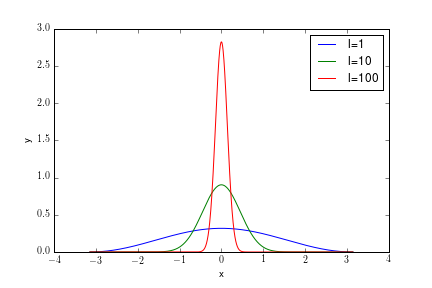
\includegraphics[width=0.40\textwidth]{figs/hk.png}}
\end{center}
\caption{\label{fig:hl} The function $h_\ell(x)$ for increasingly large values of $\ell$.}
\end{figure}

\noindent
To demonstrate the completeness of sines and cosines\footnote{This proof taken from http://web.mit.edu/jorloff/www/18.03-esg/notes/fourier-complete.pdf} we construct a peculiar but useful set of functions defined for $\ell=1,2,3,...$:
\begin{displaymath}
h_\ell(x) = c_\ell \left(\frac{1 + \cos(x)}{2}\right)^\ell
\end{displaymath}
We chose each factor $c_\ell$ such that:
\begin{displaymath}
\int_{-\pi}^{\pi} h_\ell(x) = 1
\end{displaymath}
The shape of $h_\ell$ is shown in Fig.~\ref{fig:hl}.  As $\ell$ increases, $h_\ell$ becomes more and more narrow at $x=0$, while the normalization is as in Equation~\ref{eqn:norm}.  It looks more and more like the delta function:
\begin{displaymath}
\lim_{\ell \to \infty} h_\ell(x) = \delta(x)
\end{displaymath}
It has one other important feature:  $h_\ell(x)$ is simply a sum of cosines of $nx$ with coefficients that don't depend on $x$.  To see how this can be, note that we can always turn a product of cosines into a sum via the trigonometric identity:
\begin{displaymath}
\cos \alpha \cos \beta = \frac{1}{2} \{\cos(\alpha - \beta) + \cos(\alpha + \beta)\}.
\end{displaymath}
So, for instance, we can write:
\begin{eqnarray*}
h_2(x) &=& \frac{c_2}{4} + \frac{c_2\cos(x)}{2}+\frac{c_2\cos^2(x)}{4} \\
           &=& \frac{3\,c_2}{8} + \frac{c_2\cos(x)}{2}+\frac{c_2\cos(2x)}{8}
\end{eqnarray*}
This property implies that the function $h_\ell(x-a)$ for some constant $a$ is simply a sum of {\em both} sines and cosines of $nx$ with coefficients that don't depend on $x$, as:
\begin{displaymath}
\cos(nx-na) = \cos(nx)\cos(na) + \sin(nx)\sin(na).
\end{displaymath}

With this technology in hand we are ready to demonstrate the completeness of the sines and cosines.   
For simplicity, it suffices to consider only functions with period $L=2\pi$ (i.e. $k_n=n$).  The general case can then be inferred by transformation of coordinates.  Consider a real function $f(x)$ which is periodic for $L=2\pi$.  For now just define the function $F(x)$ to be the infinite series:
\begin{eqnarray}
F(x) \equiv a_0 + \sum_{n=1}^{\infty}  \left\{ a_n \, \cos(n x ) + b_n \, \sin(n x ) \right\}.
\end{eqnarray}
This is the compact form of the Fourier Series for this special case $L=2\pi$, so $k_n = n$.
We assume the coefficients are determined in the usual way:
\begin{eqnarray*}
a_n &=& \frac{2}{L} \int_{-\frac{L}{2}}^{\frac{L}{2}} 
f(x) \cos(n x) \, dx  \\
b_n &=& \frac{2}{L} \int_{-\frac{L}{2}}^{\frac{L}{2}} 
f(x) \sin(n x) \, dx.
\end{eqnarray*}
We need to show that $F(x) = f(x)$, or 
\begin{displaymath}
g(x) = F(x) - f(x) = 0
\end{displaymath}
The proof hinges on the fact that $F(x)$ and $f(x)$ have the same Fourier coefficients, so that:
\begin{eqnarray*}
\int_{-\pi}^{\pi} g(x) \sin(nx) dx &=& \int_{-\pi}^{\pi} F(x) \sin(nx) dx -  \int_{-\pi}^{\pi} f(x) \sin(nx) dx \\
&=& b_n - b_n \\
&=& 0 \\
\int_{-\pi}^{\pi} g(x) \cos(nx) dx &=& \int_{-\pi}^{\pi} F(x) \cos(nx) dx -  \int_{-\pi}^{\pi} f(x) \cos(nx) dx \\
&=& a_n - a_n \\
&=& 0 
\end{eqnarray*}
This shows that the integral of $g(x)$ times any sine or cosine is zero.  But our special function $h_\ell(x-a)$ function is just a sum of sines and cosines of $nx$ for any value of $a$.  This means that:
\begin{eqnarray*}
\int_{-\pi}^{\pi} h_\ell(x-a) g(x) dx &=& 0 \\
\end{eqnarray*}
If we take the limit as $\ell \to \infty$, we obtain:
\begin{eqnarray*}
\int_{-\pi}^{\pi} \delta(x-a) g(x) dx &=& 0 \\
g(a) &=& 0 \\
\end{eqnarray*}
Since this is true for any value of $a$, we have $g(x) = 0$ and so $F(x) = f(x)$.

\end{document}


\subsection{The orthogonality and completeness of the complex exponential function}

The first thing we need to show is that:
\begin{equation} \label{eqn:delta}
\frac{1}{2\pi} \int_{-\infty}^{\infty} \exp(ikx) \, dk = \delta(x)
\end{equation}
To see this we first calculate:
\begin{eqnarray*} \label{eqn:delta}
\frac{1}{2\pi} \int_{-a}^{a} \exp(ikx) \, dk &=& \frac{1}{2\pi} \, \frac{\exp(iax)-\exp(-iax)}{ix}\\
&=& \frac{1}{\pi} \, \frac{\sin(ax)}{x} \\
&=& \frac{a}{\pi} \, {\rm sinc}(ax)
\end{eqnarray*}
An integration shows that:
\begin{eqnarray}
\int_{-\infty}^{\infty} \frac{a}{\pi} \, {\rm sinc}(ax) \, dx = 1
\end{eqnarray}
exactly as needed for Equation~\ref{eqn:norm}.

Fig.~\ref{fig:sinc} shows that this function peaks at zero and becomes more and more narrow for progressively larger values of $a$.  Since it has the correct normalization, we conclude that:
\begin{eqnarray*}
\frac{1}{2\pi} \int_{-\infty}^{\infty} \exp(ikx) \, dk &=& \lim_{a\to\infty} \frac{1}{2\pi} \int_{-a}^{a} \exp(ikx) \, dk \\
&=& \lim_{a\to\infty} \frac{a}{\pi} \, {\rm sinc}(ax) \\ 
&=& \delta(x)
\end{eqnarray*}

\begin{figure}[thb]
\begin{center}
{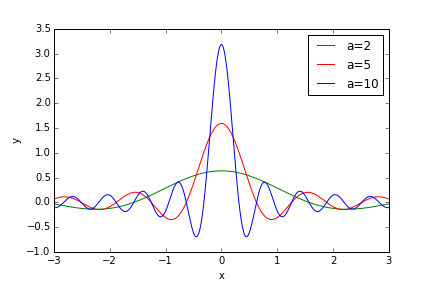
\includegraphics[width=0.40\textwidth]{figs/sinc.png}}
\end{center}
\caption{\label{fig:sinc} The function $a \, {\rm sinc}(ax)/\pi$ for progressively larger values of $a$.  As $a \to \infty$, this function approaches the delta function $\delta(x)$.}
\end{figure}

We are now fully equip to show that the complex exponential functions:
\begin{equation*}
e_k = \frac{1}{\sqrt{2\pi}} \exp(i k x)
\end{equation*}
are orthonormal.  Calculating the inner product
\begin{eqnarray*}
\braket{e_k, e_{k'}} &=& \int_{-\infty}^{\infty} \frac{1}{\sqrt{2 \pi}}  \exp(-ikx) \frac{1}{\sqrt{2 \pi}}  \exp(ik'x) \, dx \\
                               &=& \frac{1}{2 \pi} \int_{-\infty}^{\infty} \exp\{i(k'-k)x\} \, dx \\
                               &=& \delta(k-k')
\end{eqnarray*}
where we have used Equation~\ref{eqn:delta} but with the roles of $x$ and $k$ exchanged.
To prove completeness, we can now show that:
\begin{eqnarray*}
\Psi(x) &=& \int_{-\infty}^{\infty} \Psi(x') \, \delta(x-x') \, dx' \\
&=& \int_{-\infty}^{\infty} f(x') \left\{ \frac{1}{2 \pi} \int_{-\infty}^{+\infty} \exp\{ik(x-x')\} \, dk \right\} \, dx' \\
&=& \frac{1}{\sqrt{2 \pi}} \int_{-\infty}^{\infty} \left\{ \frac{1}{\sqrt{2 \pi}} \int_{-\infty}^{+\infty} f(x') \exp(-ikx') \, dx' \right\}  \exp(ikx) \, dk \\
&=& \frac{1}{\sqrt{2 \pi}} \int_{-\infty}^{\infty} \widetilde{\Psi}(k)  \exp(ikx) \, dk \\
\end{eqnarray*}
where:
\begin{eqnarray*}
\widetilde{\Psi}(k) &=& \frac{1}{\sqrt{2\pi}} \int_{-\infty}^{\infty} \Psi(x) \, \exp(-ikx) \, dx \\
\end{eqnarray*}



\end{document}





